\documentclass[12pt]{article}
\usepackage[margin=1in]{geometry}
\usepackage{amsmath,amsthm,amssymb,amsfonts}
\usepackage{bm}
\usepackage{graphicx}

\newcommand{\N}{\mathbb{N}}
\newcommand{\Z}{\mathbb{Z}}


\begin{document}


\title{Homework 3}
\author{Yasheng Sun}
\date{}

\maketitle
[The project code is on my github https://github.com/sunyasheng/Neural-Network-Assignment]
\section{Solution}
In this assignment, we compared the capabilities of feedforward neural network and CNN. 

\subsection{Network Structure}
The feedforward neural network and CNN structure are shown below. Left is for feedforward network, right is CNN.
\begin{center}
  Graph model for feedforward network and CNN model.
  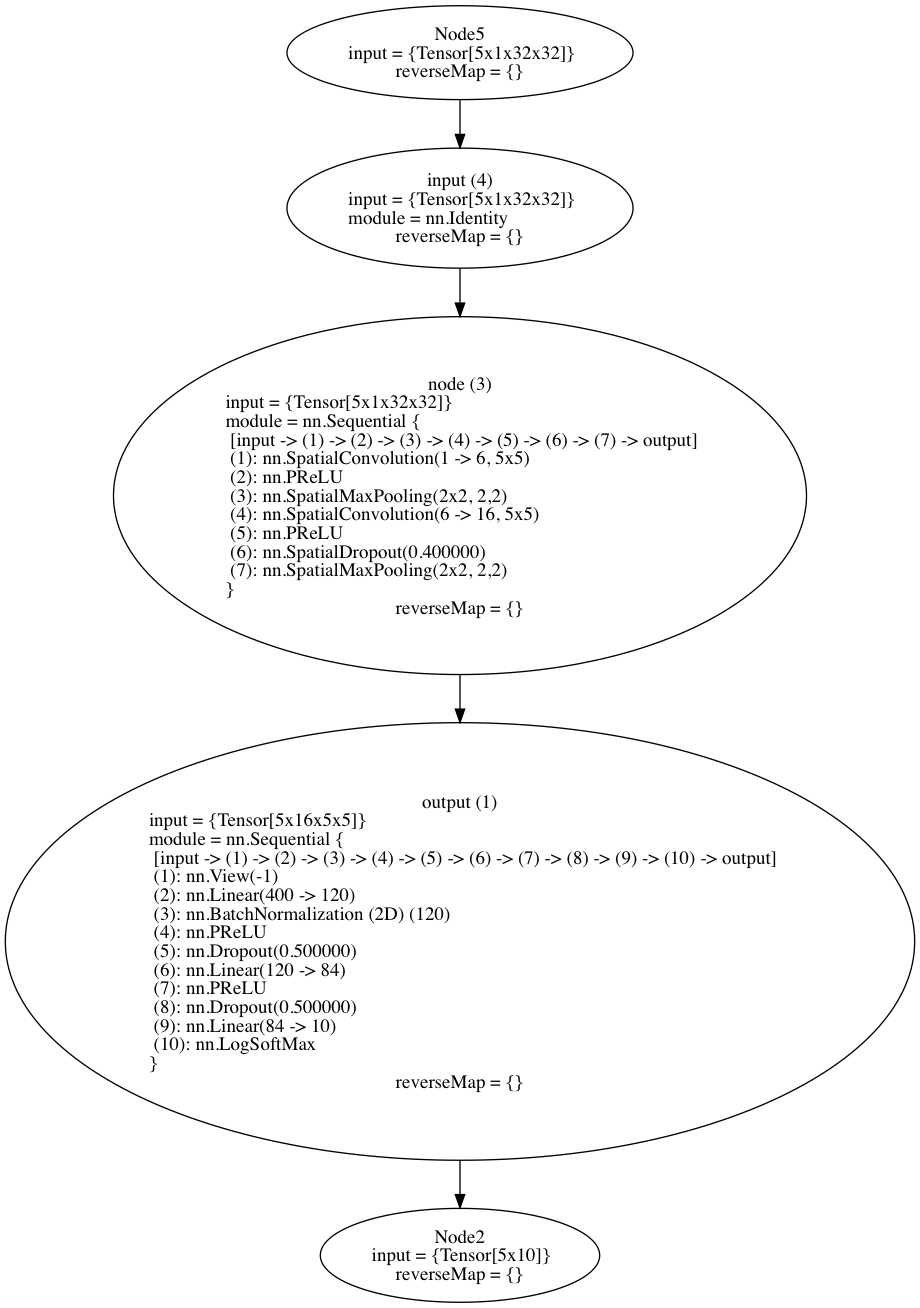
\includegraphics[angle = 0, width = .48\textwidth]{./model_structure/cnn_model.png}
  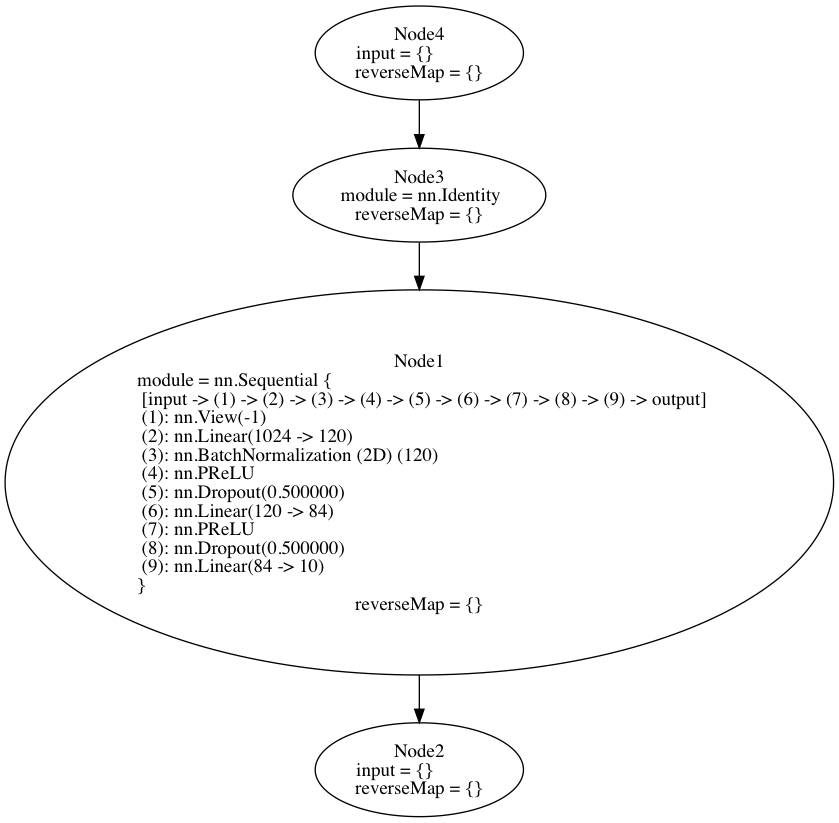
\includegraphics[angle = 0, width = .48\textwidth]{./model_structure/mlp_model.png}
\end{center}

\subsection{Training Time}
The training process runs on Mac OS 10.12.6 with 2.5 GHz Intel Core i5 CPU and 10 GB 1600 MHz DDR3. For the feedforward structure, it takes 6 minutes to run 6000 iterations while it take 40 minutes for CNN.

\subsection{Training Error and Accurary}
Both of these two networks perform well in test dataset. It seems that the CNN behaves more stable in training process. This is because CNN have the sharing weights technique which avoids overfiting to some degree. Left is for feedforward network, right is CNN. 
\begin{center}
  Evolution of accuracy on training dataset in 6000 iterations.\\
  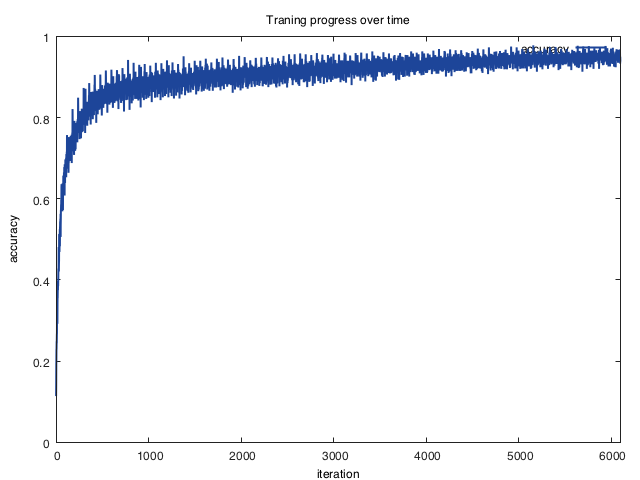
\includegraphics[angle = 0, width = .48\textwidth]{./train_images/mlpnet_Mnist_accuracy.png}
  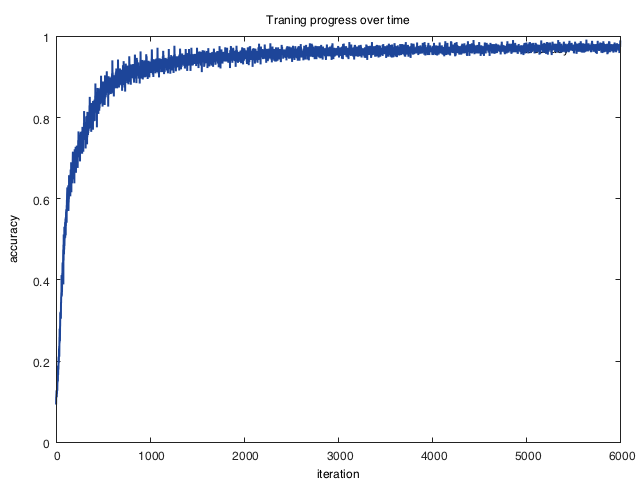
\includegraphics[angle = 0, width = .48\textwidth]{./train_images/lenet_Mnist_accuracy.png}
\end{center}
\begin{center}
  Evolution of CrossEntropy loss on training dataset in 6000 iterations.\\
  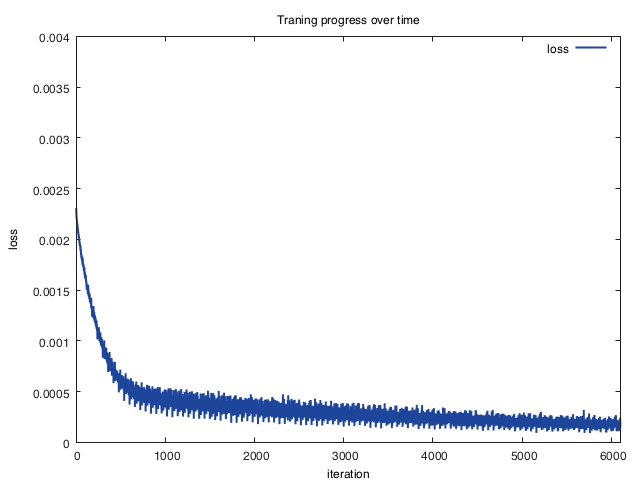
\includegraphics[angle = 0, width = .48\textwidth]{./train_images/mlpnet_Mnist_loss.png}
  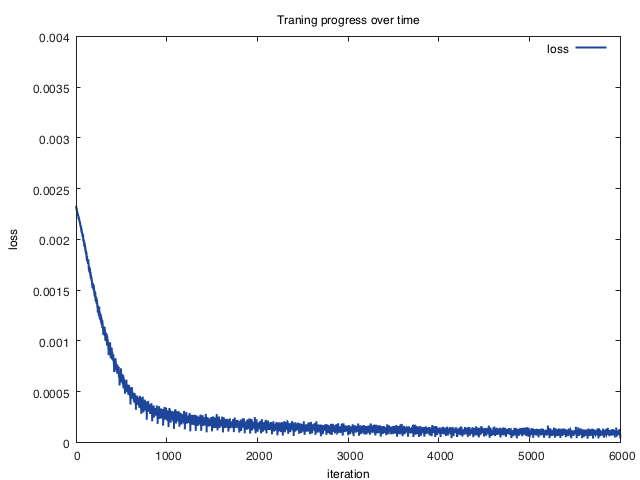
\includegraphics[angle = 0, width = .48\textwidth]{./train_images/lenet_Mnist_loss.png}
\end{center}
\subsection{Testing Error}
We test the trained model in testing dataset at 6 stages. The test accuracy is shown below. Left is for feedforward network, right is CNN. Obviously, the CNN performs much better than feedforward network. For CNN, the accuracy decreases with iteration, which may be caused by overfiting in training stage. For feedforward network, there must be some magic behind there. God knows why the accuracy decreases first and then increases gradually.
\begin{center}
  Evolution of accuracy on testing dataset at 6 stages.
  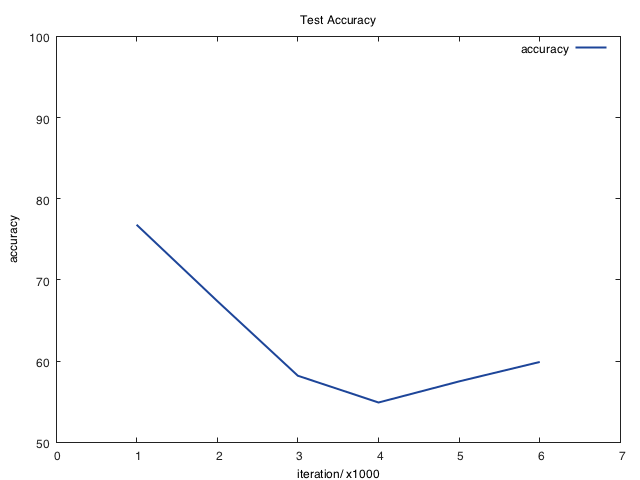
\includegraphics[angle = 0, width = .48\textwidth]{./test_images/mlp_testAccuracy.png}
  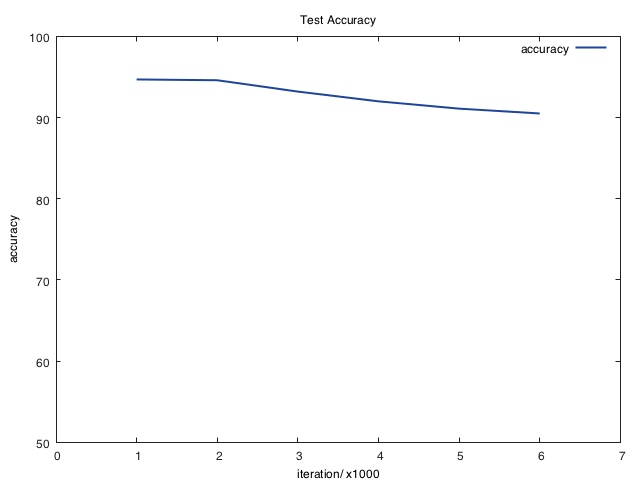
\includegraphics[angle = 0, width = .48\textwidth]{./test_images/lenet_testAccuracy.png}
\end{center}

\section{Feature Visualization}
Extracted Features are shown below. Left is the feature extracted in lower layers while right is the feature extracted in higher layers. It seems that the extracted features keep the whole shape of the original image. 
\begin{center}
  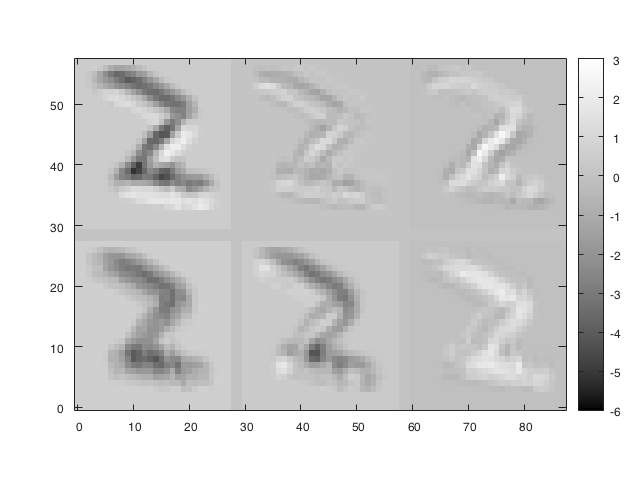
\includegraphics[angle = 0, width = .48\textwidth]{./feature_images/label_2_feature_1.png}
  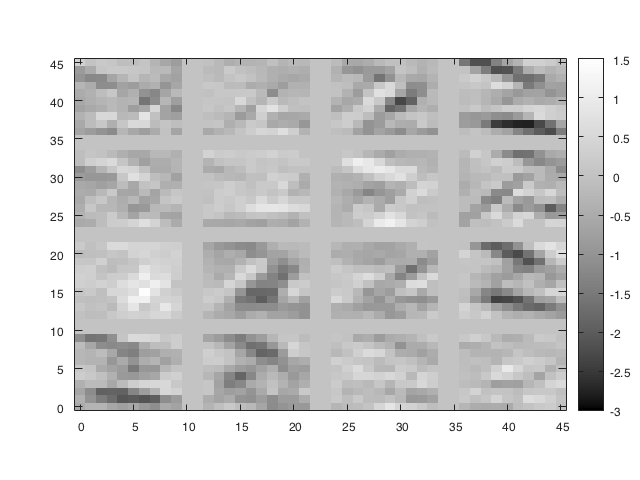
\includegraphics[angle = 0, width = .48\textwidth]{./feature_images/label_2_feature_2.png}
\end{center}
\section{Note}
The usage of the code is illustrated in ReadMe which is also on my github.

\end{document}